\documentclass[12pt]{article}
\usepackage[utf8]{inputenc}

\usepackage{lmodern}

\usepackage{enumitem}
\usepackage[margin=2cm]{geometry}

\usepackage{amsmath, amsfonts, amssymb}
\usepackage{graphicx}
%\usepackage{subfigure}
\usepackage{tikz}
\usepackage{pgfplots}
\usepackage{multicol}

\usepackage{comment}
\usepackage{url}
\usepackage{calc}
\usepackage{subcaption}
\usepackage[indent=0pt]{parskip}
\usepackage{animate}

\usepackage{array}
\usepackage{blkarray,booktabs, bigstrut}
\usepackage{bigints}

\pgfplotsset{compat=1.16}

% MATH commands
\newcommand{\ga}{\left\langle}
\newcommand{\da}{\right\rangle}
\newcommand{\oa}{\left\lbrace}
\newcommand{\fa}{\right\rbrace}
\newcommand{\oc}{\left[}
\newcommand{\fc}{\right]}
\newcommand{\op}{\left(}
\newcommand{\fp}{\right)}

\newcommand{\bi}{\mathbf{i}}
\newcommand{\bj}{\mathbf{j}}
\newcommand{\bk}{\mathbf{k}}
\newcommand{\bF}{\mathbf{F}}

\newcommand{\mR}{\mathbb{R}}

\newcommand{\ra}{\rightarrow}
\newcommand{\Ra}{\Rightarrow}

\newcommand{\sech}{\mathrm{sech}\,}
\newcommand{\csch}{\mathrm{csch}\,}
\newcommand{\curl}{\mathrm{curl}\,}
\newcommand{\dive}{\mathrm{div}\,}

\newcommand{\ve}{\varepsilon}
\newcommand{\spc}{\vspace*{0.5cm}}

\DeclareMathOperator{\Ran}{Ran}
\DeclareMathOperator{\Dom}{Dom}

\newcommand{\exo}[1]{\noindent\textcolor{red}{\fbox{\textbf{Problem {#1}}}\hrulefill}\\\\ }
\newcommand{\qu}[4]{\noindent\textcolor{#4}{\fbox{\textbf{Section {#1} | Problem {#2}}} \hrulefill{{\fbox{\textbf{{#3} Points}}}}\\}}

\newcommand{\semester}{Fall 2023}

\newcommand{\CVup}{%

\begin{tikzpicture}
\draw[black, <->, >=latex] (-0.33, 0.5) .. controls (-0.125, 0) and (0.125, 0) .. (0.33, 0.5);
\end{tikzpicture}}

\newcommand{\CVupInc}{%
\begin{tikzpicture}
\draw[black, ->, >=latex] (0,0) .. controls (0.2, 0) and (0.4, 0.2) .. (0.5, 0.5);
\end{tikzpicture}}

\newcommand{\CVupDec}{%
\begin{tikzpicture}[rotate=270]
\draw[black, ->, >=latex] (0,0) .. controls (0.2, 0) and (0.4, 0.2) .. (0.5, 0.5);
\end{tikzpicture}}

\newcommand{\CVdown}{%
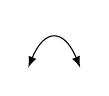
\begin{tikzpicture}
\draw[black, <->, >=latex] (-0.33, -0.5) .. controls (-0.125, 0) and (0.125, 0) .. (0.33, -0.5);
\end{tikzpicture}}

\newcommand{\CVdownInc}{%
\begin{tikzpicture}
\draw[black, ->, >=latex] (-0.5, -0.5) .. controls (-0.5, -0.3) and (-0.5, -0.1) .. (0,0);
\end{tikzpicture}}

\newcommand{\CVdownDec}{%
\begin{tikzpicture}[rotate=-90]
\draw[black, ->, >=latex] (-0.5, -0.5) .. controls (-0.5, -0.3) and (-0.5, -0.1) .. (0,0);
\end{tikzpicture}}

\begin{document}
	\noindent \hrulefill \\
	MATH-244 \semester \hfill Practice Problems Solutions\\
	Section 15.9 \hfill Pierre-Olivier Paris{\'e} \\\vspace*{-1cm}
	
	\noindent\hrulefill
	
	\spc	

	\exo{10}
	\\
	The transformation is given by $T(u, v) = (au, bv)$ and so $x(u, v) = au$ and $y(u, v) = bv$. We then see that $x/a = u$ and $y/b = v$. 
	
	The boundary of the region $S$ is the circle $u^2 + v^2 = 1$. Replacing $u$ by $x/a$ and $v$ by $y/b$, we get the equation $(x/a)^2 + (y/b)^2 = 1$. This is an ellipse centered at the origin. Thus, the region $R = T(S)$ is the interior of the ellipse given by the equation $(x/a)^2 + (y/b)^2 = 1$.
	
	\spc 
	
	\exo{12}
	\\
	Here's an illustration of the parallelogram.
		\begin{figure}[h]
		\centering
		\includegraphics[scale=0.4]{prob12_15-9.png}
		\end{figure}
	
	The equation of the line joining the points $(4, 3)$ and $(2, 4)$ is $y + x/2 = 5$. The equation of the line joining the points $(-2, 1)$ and $(0, 0)$ is $y + x/2 = 0$. The equation of the line joining $(2, 4)$ and $(-2, 1)$ is $y - (3/4)x = 5/2$. The equation of the line joining $(0,0)$ and $(4, 3)$ is $y - (3/4)x = 0$.
	
	Take $u = y - (3/4)x$ and $v = y + x/2$. So
		\begin{itemize}
		\item The line passing through $(4, 3)$ and $(2, 4)$ becomes $0 \leq u \leq 5/2$ and $v = 5$.
		\item The line passing through $(2, 4)$ and $(-2, 1)$ becomes $u = 5/2 $ and $0 \leq v \leq 5$.
		\item The line passing through $(-2, 1)$ and $(0, 0)$ becomes $0 \leq u \leq 5/2$ and $v = 0$.
		\item The line passing through $(0, 0)$ and $(4, 3)$ becomes $u = 0$ and $0 \leq v \leq 5$.
		\end{itemize}
	These new lines in the $uv$-plane are the boundary curves of the following rectangle:
		\begin{figure}[h]
		\centering
		\includegraphics[scale=0.16]{rectangle-15-9_Prob12.png}
		\caption{$[0, 5/2] \times [0, 5]$}
		\end{figure}
	
	\spc 
	
	\exo{18}
	\\
	The ellipse can be rewritten as
		\begin{align*}
		x(x-y) + y^2 = 2 .
		\end{align*}
	Replacing $x$ and $y$ by the transformations, we have
		\begin{align*}
		(\sqrt{2} u - \sqrt{2/3} v)(-2\sqrt{2/3} v) + u^2 + 4uv/\sqrt{3} + 2v^2/3 = 2 \iff u^2 + 2v^2 = 2 \iff (u/\sqrt{2})^2 + v^2 = 1 .
		\end{align*}
	So the region $R$ bounded by the ellipse $x^2 + xy + y^2 = 2$ is the image of the region $S$ bounded by the ellipse $u^2/2 + v^2 = 1$. The description of $S$ is
		\begin{align*}
		S = \{ (u, v) \, : \, u^2/2 + v^2 \leq 1 \} .
		\end{align*}
	The Jacobian of the transformation is
		\begin{align*}
		\left| \begin{matrix}
		x_u & x_v \\
		y_u & y_v
		\end{matrix}
		\right| = \left| \begin{matrix}
		\sqrt{2} & -\sqrt{2/3} \\
		\sqrt{2} & \sqrt{2/3}
		\end{matrix}
		\right| = 4/\sqrt{3} .
		\end{align*}
	So, the integral over $R$ become
		\begin{align*}
		\iint_R x^2 - xy + y^2 \, dA = (4/\sqrt{3})\iint_S u^2/2 + v^2 \, du dv .
		\end{align*}
	We will need another change of variable. Take $u = \sqrt{2} r \cos \theta$ and $v = r \sin \theta$. In these coordinates, we see that $0 \leq r \leq 1$ and $0 \leq \theta \leq 2\pi$. The Jacobian of these transformation is
		\begin{align*}
		\left| \begin{matrix}
		u_r & u_\theta \\
		v_r & v_\theta
		\end{matrix} \right| = 
		\left| \begin{matrix}
		\sqrt{2} \cos \theta & - \sqrt{2} r \sin \theta \\
		\sin \theta & r \cos \theta
		\end{matrix} \right| = r \sqrt{2} .
		\end{align*}
	So, we get
		\begin{align*}
		\iint_S u^2/2 + v^2 \, dudv = \int_0^{2\pi} \int_0^1 r^3 \sqrt{2} \, dr d\theta = \pi \sqrt{2} /2 .
		\end{align*}

\end{document}